\documentclass[russian,]{article}
\usepackage[]{amsmath}
\usepackage{amssymb,amsmath}
\usepackage{ifxetex,ifluatex}
\usepackage{fixltx2e} % provides \textsubscript
\ifnum 0\ifxetex 1\fi\ifluatex 1\fi=0 % if pdftex
  \usepackage[T1, T2A]{fontenc}
  \usepackage[utf8]{inputenc}
\else % if luatex or xelatex
  \ifxetex
    \usepackage{mathspec}
  \else
    \usepackage{fontspec}
  \fi
  \defaultfontfeatures{Ligatures=TeX,Scale=MatchLowercase}
\fi
% use upquote if available, for straight quotes in verbatim environments
\IfFileExists{upquote.sty}{\usepackage{upquote}}{}
% use microtype if available
\IfFileExists{microtype.sty}{%
\usepackage[]{microtype}
\UseMicrotypeSet[protrusion]{basicmath} % disable protrusion for tt fonts
}{}
\PassOptionsToPackage{hyphens}{url} % url is loaded by hyperref
\usepackage[unicode=true]{hyperref}
\hypersetup{
            pdfborder={0 0 0},
            breaklinks=true}
\urlstyle{same}  % don't use monospace font for urls
\ifnum 0\ifxetex 1\fi\ifluatex 1\fi=0 % if pdftex
  \usepackage[shorthands=off,main=russian]{babel}
\else
  \usepackage{polyglossia}
  \setmainlanguage[]{}
\fi
\usepackage{longtable,booktabs}
% Fix footnotes in tables (requires footnote package)
\IfFileExists{footnote.sty}{\usepackage{footnote}\makesavenoteenv{long table}}{}
\usepackage{graphicx,grffile}
\makeatletter
\def\maxwidth{\ifdim\Gin@nat@width>\linewidth\linewidth\else\Gin@nat@width\fi}
\def\maxheight{\ifdim\Gin@nat@height>\textheight\textheight\else\Gin@nat@height\fi}
\makeatother
% Scale images if necessary, so that they will not overflow the page
% margins by default, and it is still possible to overwrite the defaults
% using explicit options in \includegraphics[width, height, ...]{}
\setkeys{Gin}{width=\maxwidth,height=\maxheight,keepaspectratio}
\IfFileExists{parskip.sty}{%
\usepackage{parskip}
}{% else
\setlength{\parindent}{0pt}
\setlength{\parskip}{6pt plus 2pt minus 1pt}
}
\setlength{\emergencystretch}{3em}  % prevent overfull lines
\providecommand{\tightlist}{%
  \setlength{\itemsep}{0pt}\setlength{\parskip}{0pt}}
\setcounter{secnumdepth}{0}
% Redefines (sub)paragraphs to behave more like sections
\ifx\paragraph\undefined\else
\let\oldparagraph\paragraph
\renewcommand{\paragraph}[1]{\oldparagraph{#1}\mbox{}}
\fi
\ifx\subparagraph\undefined\else
\let\oldsubparagraph\subparagraph
\renewcommand{\subparagraph}[1]{\oldsubparagraph{#1}\mbox{}}
\fi

% set default figure placement to htbp
\makeatletter
\def\fps@figure{htbp}
\makeatother

\usepackage[a4paper,left=20mm,right=10mm,top=20mm,bottom=20mm]{geometry}

\usepackage{amsgen, amsmath, amstext, amsbsy, amsopn, amsfonts, amsthm, thmtools,  amssymb, amscd, mathtext, mathtools}
\usepackage{versions}

\usepackage{float}
\restylefloat{table}

\usepackage{xfrac}

\usepackage{pifont}

\usepackage{xspace}

% Explain
\newcommand{\expl}[2]{\underset{\mathclap{\overset{\uparrow}{#2}}}{#1}}
\newcommand{\explup}[2]{\overset{\mathclap{\underset{\downarrow}{#2}}}{#1}}
\newcommand{\obrace}[2]{\overbrace{#1}^{#2}}
\newcommand{\ubrace}[2]{\underbrace{#1}_{#2}}

% Arrows
\newcommand{\Then}{\Rightarrow}
\newcommand{\Iff}{\Leftrightarrow}
\newcommand{\When}{\Leftarrow}
\newcommand{\Bydef}{\rightleftharpoons}
%\newcommand{\Divby}{\raisebox{-2pt}{\vdots}}
\DeclareRobustCommand{\Divby}{%
  \mathrel{\text{\vbox{\baselineskip.65ex\lineskiplimit0pt\hbox{.}\hbox{.}\hbox{.}}}}%
}

\DeclareMathOperator{\Char}{char}
\DeclareMathOperator{\Ker}{Ker}
\DeclareMathOperator{\Quot}{Quot}
\DeclareMathOperator{\Gal}{Gal}
\DeclareMathOperator{\Aut}{Aut}

% Mathbbs
\newcommand{\N}{\mathbb{N}}
\newcommand{\Z}{\mathbb{Z}}
\newcommand{\Q}{\mathbb{Q}}
\newcommand{\R}{\mathbb{R}}
\renewcommand{\C}{\mathbb{C}}

\renewcommand{\~}{\sim}
\renewcommand{\phi}{\varphi}
\newcommand{\ol}{\overline}
\newcommand{\cmark}{\ding{51}}
\newcommand{\xmark}{\ding{55}}
\newcommand{\y}{\cmark}
\newcommand{\x}{\xmark}

% Кавычки
\newcommand{\lgq}{\guillemotleft\nobreak\ignorespaces}
\newcommand{\rgq}{\guillemotright\xspace}

% Consider changing to sfrac
\newcommand{\bigslant}[2]{{\raisebox{.2em}{$#1$}\left/\raisebox{-.2em}{$#2$}\right.}}

\makeatletter
\newenvironment{sqcases}{%
  \matrix@check\sqcases\env@sqcases
}{%
  \endarray\right.%
}
\def\env@sqcases{%
  \let\@ifnextchar\new@ifnextchar
  \left\lbrack
  \def\arraystretch{1.2}%
  \array{@{}l@{\quad}l@{}}%
}
\makeatother

\makeatletter
\newenvironment{nocases}{%
  \matrix@check\sqcases\env@sqcases
}{%
  \endarray\right.%
}
\def\env@nocases{%
  \let\@ifnextchar\new@ifnextchar
  \def\arraystretch{1.2}%
  \array{@{}l@{\quad}l@{}}%
}
\makeatother

\newcommand{\nopandoc}[1]{#1} % hide LaTeX code from pandoc
\nopandoc{
	\let\Begin\begin
	\let\End\end
}


% Styles
\declaretheoremstyle[notefont=\bfseries,notebraces={}{},headpunct={},%
postheadspace={5px},headformat={\makebox[0pt][r]{\NAME\ \NUMBER\ }\setbox0\hbox{\ }\hspace{-\the\wd0}\NOTE}]{problemstyle}
\declaretheorem[style=problemstyle,numbered=no,name=№]{problem}

\declaretheoremstyle[notefont=\bfseries,notebraces={}{},headpunct={ },postheadspace={0px},qed=$\blacktriangleleft$,
headformat={\makebox[0pt][r]{\NAME\ }\setbox0\hbox{\ }\hspace{-\the\wd0}\NOTE},]{solutionstyle}
\declaretheorem[style=solutionstyle,numbered=no,name=$\blacktriangleright$]{solution}

\declaretheoremstyle[notefont=\bfseries,notebraces={}{},headpunct={.},postheadspace={4px}]{definitionstyle}
\declaretheorem[style=definitionstyle,numbered=yes,name=Опр.]{defn}



\date{}

\begin{document}

\begin{problem}[1 (1.1)]
Для любых $a,b,c \in K$ выполнены равенства
\end{problem}

\(\forall a, b, c \in K\):

\begin{enumerate}
\def\labelenumi{\alph{enumi})}
\i
  \(a0=0a=0\)
  \begin{solution}
  \(a0=a(0+0)=a0+a0 \Then a0=0\)

  \(0a=0\) --- аналогично.
  \end{solution}
\i
  \(a(-b)=(-a)b=-ab\)
  \begin{solution}
  \(0=a0=a(b-b)=ab+a(-b) \Then -ab = a(-b)\)
  \end{solution}
\i
  \((a-b)c = ac-bc\) и \(a(b-c)=ab-ac\)
  \begin{solution}
  \((a-b)c+bc = (a-b+b)c=ac \Then (a-b)c = ac-bc\)

  \(a(b-c)+ac=a(b-c+c)=ab \Then a(b-c)=ab-ac\)
  \end{solution}
\end{enumerate}

\begin{problem}[2(1.2)]
\end{problem}

\begin{enumerate}
\def\labelenumi{\alph{enumi})}
\i
  В кольце не может быть двух различных единиц.
  \begin{solution}
  \(1_1 \ubrace{=}{\text{т. к.} 1_2 \text{--- единица}} 1_1 \cdot 1_2 \ubrace{=}{\text{т. к.} 1_1 \text{--- единица}} 1_2\)
  \end{solution}
\i
  Пусть кольцо с единицей содержит не меньше двух элементов. Тогда \(1 \neq 0\).
  \begin{solution}
  \(\forall a \in K\ a \ubrace{=}{\text{св-во 1}} a \cdot e \ubrace{=}{\text{св-во 0}} 0\)
  \end{solution}
\i
  Может ли элемент ассоциативного кольца иметь более одного обратного элемента?
  \begin{solution}
  Пусть \(a_1 \ne a_2\) --- обратные к \(a\) элементы. Тогда
  \(a_1 a a_2 = \begin{cases} a_1 \cdot 1 = a_1 \\ 1 \cdot a_2 = a_2 \end{cases}\)

  Получается, они равны.
  \end{solution}
\end{enumerate}

\begin{problem}[3(1.3, 2.4)]
Уметь отвечать на вопросы: является ли данное кольцо K коммутативным? ассоциативным?кольцом с единицей? область целостности? поле? евклидово кольцо? Какие в K есть обратимые элементы? неразложимые? простые?
\end{problem}

\begin{problem}[4 (2.1(в))]
Обратимый элемент кольца не может быть делителем нуля.
\end{problem}

\begin{solution}
Пусть \(a \in K\) обратим, \(\exists a^{-1} \in K: aa^{-1} = 1\). Если \(a\) --- делитель нуля, то \(\exists 0 \ne b \in K: ab=0\). Тогда \(a^{-1} a b = \begin{cases} a^{-1} \cdot 0 = 0 \\ 1 \cdot b = b \ne 0 \end{cases}\).
Противоречие.
\end{solution}

\begin{problem}[5(2.1(д))]
Если $K$ --- кольцо без делителей нуля, то возможно сокращение: если $ac=bc$ и $c \neq 0$, то $a=b$.
\end{problem}

\begin{solution}
\(ac=bc \Iff (a-b)c=0 \Then\) т. к. нет делителей нуля и \(c \ne 0\), д. б. \(a-b=0\), т. е. \(a=b\).
\end{solution}

\begin{problem}[6(2.1(г))]
В конечном коммутативном кольце если ненулевой элемент не является делителем нуля, то он обратим.
\end{problem}

\begin{solution}
Кольцо конечно \(\Then\) его элементы можно занумеровать: \(a_1, \dots, a_n\). Элементы \(a\cdot a_1, \dots, a \cdot a_n\) должны быть все разные (иначе \(\forall i \ne j, a \ne 0 \ a\cdot a_i = a \cdot a_j \Then \ubrace{a}{\ne 0} \ubrace{(a_i-a_j)}{\ne 0\text{, т. к. }i \ne j} = 0\), т. е. \(a\) --- делитель нуля).

Тогда \(\exists i: a \cdot a_i = 1\), т. к. \(1 \in K\) (т. е. \(a\cdot a_1, \dots, a \cdot a_n\) --- \(n\) разных элементов кольца, а в кольце всего \(n\) элементов; значит, какое-то \(aa_i\) должно быть \(1\)).
\end{solution}

\begin{problem}[7]
Конечная область целостности (состоящая из более чем одного элемента) --- поле.
\end{problem}

\begin{solution}
В области целостности нет делителей нуля, а если в конечном коммутативном кольце элемент --- не делитель нуля, то он обратим (№6). Т. е. все элементы обратимы.

Имеем \(\ge 2\) элементов по условию.
\end{solution}

\begin{problem}[8]
Множество $K^*$ обратимых элементов коммутативного кольца K является группой по умножению. Она называется \bf{мультипликативной группой}, или \bf{группой обратимых элементов} кольца $K$.
\end{problem}

\begin{solution}
Пусть \(K\) --- кольцо, \(a, b \in K^*\). Тогда \(\exists a^{-1}, b^{-1} \in K^*\). Проверим групповые свойства.

\begin{enumerate}
\def\labelenumi{\arabic{enumi}.}
\tightlist
\i
  a(bc) = (ab)c --- ассоциативность в \(K^*\) следует из свойств кольца \(K\).
\i
  \(\exists 1 \in K^*\) (т. к. \(K^* \ne \emptyset\), \(\exists a \in K^*\), по свойству обратимости \(\exists a^{-1} \in K^*: aa^{-1} = 1\) --- единица в \(K\) будет являться единицей в \(K^*\)).
\i
  \((b^{-1}a^{-1})(ab) = (ab)(b^{-1}a^{-1})=1 \Then (ab)^{-1} = b^{-1} a^{-1} \in K^*\) --- обратимость.
\end{enumerate}

Значит, \(K^*\) --- группа по умножению.
\end{solution}

\begin{problem}[9(1.5-1.7)]
Базовые знания про комплексные числа: сложение, умножение, модуль, аргумент, извлечение корней n-ой степени.
\end{problem}

\begin{solution}
\bf{Компл'ексное число} \(z\) --- это выражение вида \(z=a+bi\), где \(a\) и \(b\) --- числа из \(\R\), а \(i\) --- \bf{мнимая единица}. По определению \(i^2=-1\).
Число \(a\) называют \bf{вещественной частью} комплексного числа \(z\) (пишется \(a={\rm Re}\,(z)\)), а число \(b\) --- \bf{мнимой частью} \(z\) (пишется \(b={\rm Im}\,(z)\)).
Комплексные числа можно складывать и умножать, \lgq раскрывая скобки и приводя подобные\rgq. Множество комплексных чисел обозначают буквой \(\C\).

Каждому комплексному числу \(z=a+bi\) сопоставим точку \((a,b)\) и вектор \((a,b)\). Длина этого вектора называется \bf{модулем} числа \(z\) и обозначается \(|z|\). Пусть \(z\ne0\).
Угол (в радианах), отсчитанный против часовой стрелки от вектора \((1,0)\) до вектора \((a,b)\), называется \bf{аргументом} числа \(z\) и обозначается \({\rm Arg}\,(z)\). Аргумент определен с точностью до прибавления числа вида \(2\pi n\), где \(n\in\Z\).

\bf{Тригонометрическая форма записи.} Для любого ненулевого комплексного числа \(z\) имеет место равенство\textbackslash{} \(z=r (\cos \varphi +i\sin \varphi )\), где \(r=|z|\), \(\varphi={\rm Arg}\,(z)\).

Для комплексного числа \(z=r(\cos\varphi+i\sin\varphi)\) и натурального числа \(n\in\N\) выполнена \bf{формула Муавра} \textbackslash{}
\(z^n=r^n(\cos n\varphi+i\sin n\varphi)\).

Для комплексного числа \(z=a+bi\), где \(a,b\in \R\) число \(\overline{z}=a-bi\) называется \bf{комплексно-сопряжённым} к \(z\). Выполнены следующие равенства:

\(|z|^2=z\overline{z}\), \(\overline{z+w} = \overline{z} + \overline{w}\), \(\overline{zw}= \overline{z}\overline{w}\).

\end{solution}

\begin{problem}[10(2.2)]
\end{problem}

\begin{enumerate}
\def\labelenumi{\alph{enumi})}
\i
  Следующие условия эквивалентны:

  \begin{enumerate}
  \def\labelenumii{(\arabic{enumii})}
  \tightlist
  \i
    \(x \sim y\);
  \i
    \(x \mid y\) и \(y \mid x\);
  \i
    множество делителей \(x\) и множество делителей \(y\) равны.
  \end{enumerate}

  \begin{solution}

  \begin{itemize}
  \tightlist
  \i
    \((1) \Then (2):\)
    \(\exists r \in K^*: x=ry \Then y|x\) по определению.
    Т. к. \(r \in K^*\), \(\exists r^{-1} \in K^*: r^{-1}x=y \Then x|y\) по определению.
  \i
    \((2) \Then (3):\)
    Пусть \(x|y, x \Divby a\). Тогда \(y = xc, x = ab\) (по опр.) \(\Then\) \(y = xc = abc = a(bc) \Then y \Divby a\).
  \i
    \((3) \Then (2):\)
    Множества делителей \(x\) и \(y\) совпадают, \(x|x \Then x\) будет во множестве делителей \(y\), т. е. \(x|y\). Симметрично, \(y|x\).
  \i
    \((2) \Then (1):\)
    \(\begin{cases} x | y \Then y = kx\\ y | x \Then x = ty \end{cases}\)
    Тогда \(y=kty \Then kt = 1\) Значит, \(k\) и \(t\) обратимы. Значит, \(x=ty, t \in K^* \Then x \~ y\) по определению.
  \end{itemize}

  \end{solution}
\i
  Отношение \(\sim\) является отношением эквивалентности.
  \begin{solution}

  \begin{enumerate}
  \def\labelenumii{\arabic{enumii}.}
  \i
    \(x\~x\), т. к. \(\exists 1 \in K^*: x=1x\)
  \i
    \(x \~ y \Then \exists r \in K^*: x = ry \Then y = r^{-1}x \Then y \~ x\)
  \i
    \(x \~ y, y \~ z \Then \begin{cases} \exists r_1 \in K^*: x=r_1 y\\ \exists r_2 \in K^*: y=r_2 z \end{cases} \Then x = \ubrace{r_1 r_2}{\in K^* \text{, т. к. }(r_1 r_2)^{-1} = r_2^{-1} r_1^{-1}} z \Then x \~ z\)
  \end{enumerate}

  \end{solution}
\end{enumerate}

\begin{problem}[11 (2.5)]
Если $a, b, k \in \Z$, $u\not \in \Q$, то $z= a+bu \in \Z[u]$ делится на $k$ тогда и только тогда, когда $a$ и $b$ делятся на $k$.
\end{problem}

\begin{solution}

\begin{itemize}
\i
  \(\Then:\)
  \(\begin{cases} a \Divby k \\ b \Divby k \end{cases} \Then \begin{cases} a = ka' \\ b = kb' \end{cases} \Then z = a+bu = ka'+kb'u=k(a'+b'u) \Then z \Divby k\)
\i
  \(\Then\):
  Пусть \(z = a + bu = ka' + kb'u\). Тогда \((a - ka') = u(b - kb')\).

  Обе части целые \(\Then\) нули, потому что \(u\) не рациональное.

  Отсюда \(\begin{cases} a = ka' \\ b = kb' \end{cases} \Then \begin{cases} a \Divby k \\ b \Divby k \end{cases}\).
\end{itemize}

\end{solution}

\begin{problem}[12(2.9 $\When$)]
$K$ — евклидово кольцо. Верно ли, что для $a \ne 0, b \in K^*$ выполнено равенство $N(ab) = N(a)$?
\end{problem}

\begin{solution}
\(b \in K^* \Then N(a) \le N(ab) \le N(abb^{-1}) = N(a)\)
\end{solution}

\begin{problem}[13 (3.2)]
Для $u=i,\omega$ и простого целого числа $p \leq 40$ выясните, существует ли $z \in D$ с $N(z)=p$. Сформулируйте гипотезу о том, какие простые целые числа являются простыми в $D$. 
\end{problem}

\begin{solution}

Выпишем все варианты \(a, b\) с нормой \(\le 40\).

\bf{Зам.} Можно опустить перебор по \(ka', kb'\) при \(k > 1\), потому что тогда обе нормы делятся на \(k^2\).

\bf{Зам.} Можно брать только натуральные, т. к. для $\Z[i]$ норма не поменяется вообще, а для $\Z[\omega] \ N =  a^2 + ab + b^2 = a^2 - a (a+b) + (a+b)^2$, т. е. норма элемента $a - b \omega$ равна норме элемента $a + (a+b) \omega$, а такие мы уже перебрали, поскольку $a+b$ --- натуральное. Для $a <0$ симметрично.

\begin{longtable}[]{@{}llll@{}}
\toprule
a & b & \(\mathbb{Z}[i], N = a^2+b^2\) & \(\mathbb{Z}[\omega], N = a^2-ab+b^2\)\tabularnewline
\midrule
\endhead
1 & 1 & 2 & 1\tabularnewline
1 & 2 & 5 & 3\tabularnewline
1 & 3 & 10 & 7\tabularnewline
1 & 4 & 17 & 13\tabularnewline
1 & 5 & 26 & 21\tabularnewline
1 & 6 & 37 & 31\tabularnewline
2 & 2 & - & -\tabularnewline
2 & 3 & 13 & 7\tabularnewline
2 & 4 & - & -\tabularnewline
2 & 5 & 29 & 19\tabularnewline
2 & 6 & - & -\tabularnewline
2 & 7 & 53 & 39\tabularnewline
3 & 3 & - & -\tabularnewline
3 & 4 & 25 & 13\tabularnewline
3 & 5 & 34 & 19\tabularnewline
3 & 6 & - & -\tabularnewline
3 & 7 & 58 & 37\tabularnewline
4 & 4 & - & -\tabularnewline
4 & 5 & 41 & 21\tabularnewline
4 & 6 & - & -\tabularnewline
4 & 7 & 65 & 37\tabularnewline
5 & 5 & - & -\tabularnewline
5 & 6 & 61 & 31\tabularnewline
5 & 7 & 74 & 39\tabularnewline
6 & 6 & - & -\tabularnewline
\bottomrule
\end{longtable}

Пользуемся утверждением с лекции: Пусть p -- простое целое, \(\forall z \in D: N(z)\ne p \Then\) p неразложим в D.

Выпишем все простые числа \(\le 40\) и вычеркнем те, которые являются нормой. Берём оставшиеся.

\begin{table}[H]
\centering
\begin{tabular}{llllll}
\multicolumn{3}{c}{$\Z[i]$} & \multicolumn{3}{c}{$\Z[\omega]$} \\
        & 2      & \x     & \y       & 2        &          \\
\y      & 3      &        &          & 3        & \x       \\
        & 5      & \x     & \y       & 5        &          \\
\y      & 7      &        &          & 7        & \x       \\
\y      & 11     &        & \y       & 11       &          \\
        & 13     & \x     &          & 13       & \x       \\
        & 17     & \x     & \y       & 17       &          \\
\y      & 19     &        &          & 19       & \x       \\
\y      & 23     &        & \y       & 23       &          \\
        & 29     & \x     & \y       & 29       &          \\
\y      & 31     &        &          & 31       & \x       \\
        & 37     & \x     &          & 37       & \x        
\end{tabular}
\end{table}

Гипотеза:
* у \(\Z[i]\) \(4k+3\)
* у \(\Z[\omega]\) \(3k+2\) или TODO.
\end{solution}

\begin{problem}[14 (3.9)]
\end{problem}

\begin{solution}

\begin{enumerate}
\def\labelenumi{\alph{enumi})}
\tightlist
\i
  \(0 \subset K, K \subset K\) --- идеалы. Они называются \bf{тривиальными}.

  \begin{itemize}
  \tightlist
  \i
    \(\{0\}\):

    \begin{enumerate}
    \def\labelenumii{\arabic{enumii}.}
    \tightlist
    \i
      Тривиальная группа по сложению:

      \begin{itemize}
      \tightlist
      \i
        Ассоциативность наследуется
      \i
        \(0\) --- нейтральный элемент, т. к. \(0+a=a+0=0 \forall a \in \{0\}\)
      \i
        \(0^{-1} = 0 = -0\)
      \end{itemize}
    \i
      Замкнутость относительно умножения:
      \(\forall a \in K 0a=0 \in \{0\}\)
    \end{enumerate}
  \i
    \(K\):

    \begin{enumerate}
    \def\labelenumii{\arabic{enumii}.}
    \tightlist
    \i
      Тривиальная группа по сложению:

      \begin{itemize}
      \tightlist
      \i
        Ассоциативность наследуется
      \i
        \(0\) --- нейтральный элемент, т. к. \(0+a=a+0=0 \forall a \in K\)
      \i
        \(a^{-1} = -a \in K\)
      \end{itemize}
    \i
      Замкнутость относительно умножения:
      \(\forall a \in K \forall b \in I=K \ ab \in I=K\) --- по свойству кольца
    \end{enumerate}
  \end{itemize}
\i
  \((a) = \{ax \mid x\in K\}\) --- \bf{главный идеал} или \bf{идеал, порождённый одним элементом}

  \begin{enumerate}
  \def\labelenumii{\arabic{enumii}.}
  \tightlist
  \i
    Подгруппа по сложению:

    \begin{itemize}
    \tightlist
    \i
      \(ax_1+ax_2=a(x_1+x_2)\in(a)\) --- замкнутость относительно сложения
    \i
      Ассоциативность наследуется
    \i
      \(0\) --- нейтральный элемент: \(ax+0=0+ax=ax\)
    \i
      \(ax+a(-x)=a(x-x)=a\cdot 0=0\)
    \end{itemize}
  \i
    Замкнутость относительно умножения:
    \(\forall b \in K \forall ax \in (a) \ b\cdot ax = bx \cdot a \in (a)\)
  \end{enumerate}
\i
  \((a_1,\ldots,a_n) = \{a_1x_1+\ldots+a_nx_n \mid x_1,\ldots,x_n \in K\}\) --- \bf{конечно-порождённый идеал}, то есть идеал, порождённый конечным количеством элементов.

  \begin{enumerate}
  \def\labelenumii{\arabic{enumii}.}
  \tightlist
  \i
    Подгруппа по сложению:

    \begin{itemize}
    \tightlist
    \i
      \((a_1x_1+\dots+a_nx_n)+(a_1y_1+\dots+a_ny_n) = a_1(x_1+y_1)+\dots+a_n(x_n+y_n) \in I\) --- замкнутость относительно сложения
    \i
      Ассоциативность наследуется
    \i
      \(0 = a_1\cdot 0+\dots+a_1\cdot0\) --- нейтральный элемент: \(ax+0=0+ax=ax\)
    \i
      \((a_1x_1+\dots+a_nx_n)+(a_1(-x_1)+\dots+a_n(-x_n))=0\)
    \end{itemize}
  \i
    Замкнутость относительно умножения:
    \(\forall y \in K \ y\cdot (a_1x_1+\dots+a_nx_n) = a_1(x_1y)+\dots+a_n(x_ny) \in I\)
  \end{enumerate}
\end{enumerate}

\end{solution}

\begin{problem}[15(3.11)]
a) Докажите, что $(a) \subset (b)$ тогда и только тогда, когда $b \mid a$.

b) Докажите, что $a \sim b$ тогда и только тогда, когда $(a)=(b)$.
\end{problem}

\begin{solution}

\begin{enumerate}
\def\labelenumi{\alph{enumi})}
\i
  \begin{itemize}
  \tightlist
  \i
    \(\When:\) \(b | a \Then \exists c: a=cb \Then ka=(kc)b \Then (a) \subset (b)\)
  \i
    \(\Then:\) \((a) \subset (b) \Then a \in (b) \Then a=cb \Then b|a\)
  \end{itemize}
\i
  \begin{itemize}
  \tightlist
  \i
    \(\Then:\) \(a \~ b \Then \begin{cases} a|b \\ b|a \end{cases} \Then (a) \subset (b) \subset (a) \Then (a) = (b)\)
  \i
    \(\When:\) \((a) = (b) \Then \begin{cases} a|b \\ b|a \end{cases} \Then a \~ b\)
  \end{itemize}
\end{enumerate}

\end{solution}

\begin{problem}[16(3.12)]
Пусть $I,J \subset K$ --- идеалы. \bf{Сумма} $I+J = \{x+y \mid x \in I,y \in J\}$ и \bf{пересечение} $I \cap J$ идеалов являются идеалами. 
\end{problem}

\begin{solution}

\begin{enumerate}
\def\labelenumi{\alph{enumi})}
\i
  \begin{enumerate}
  \def\labelenumii{\arabic{enumii}.}
  \i
    \begin{itemize}
    \tightlist
    \i
      \((x_1+y_1)+(x_2+y_2) = \ubrace{(x_1+x_2)}{\in I}+\ubrace{(y_1+y_2)}{\in J} \in I+J\)
    \i
      Ассоциативность следует.
    \i
      0 --- нейтральный.
    \i
      \((x+y)+\ubrace{(-x-y)}{\in I+J} = (x-x)+(y-y)=0\) --- обратный
    \end{itemize}
  \i
    \(\forall a \in K \Have a(x+y)=\ubrace{ax}{\in I}+\ubrace{ay}{\in J} \in I+J\)
  \end{enumerate}
\i
  \begin{enumerate}
  \def\labelenumii{\arabic{enumii}.}
  \i
    \begin{itemize}
    \tightlist
    \i
      \(x, y \in I \cap J \Then \begin{cases} x, y \in I \\ x, y \in J \end{cases} \Then \begin{cases} x + y \in I \\ x + y \in J \end{cases} \Then x+y \in I+J\)
    \i
      Ассоциативность следует.
    \i
      0 --- нейтральный
    \i
      \(x \in I\cap J \Then \begin{cases} x \in I \\ x\in J \end{cases} \Then \begin{cases} x^{-1} \in I \\ x^{-1} \in J \end{cases} \Then x^{-1} \in I+J\) --- обратный
    \end{itemize}
  \i
    \(\forall a \in K\ \forall x \in I\cap J \Have  \begin{cases} x\in I \\ x\in J \end{cases} \Then  \begin{cases} ax\in I \\ ax\in J \end{cases} \Then  ax \in I \cap J\)
  \end{enumerate}
\end{enumerate}

\end{solution}

\begin{problem}[17(3.15)]
Пусть $K \neq 0$. Докажите, что $K$ является полем тогда и только тогда, когда $K$ не содержит нетривиальных идеалов.
\end{problem}

\begin{solution}

\begin{itemize}
\i
  \(\Then:\)
  Пусть K --- поле, \(I \subset K\) --- идеал.

  \begin{itemize}
  \tightlist
  \i
    \(x = 0 \Then (x) = \{0\}\) --- тривиальный идеал.
  \i
    \(\forall x \in I, x \ne 0, \ x\) обратим по свойству поля, значит, \(I \supset (x) = (1) = K\).
  \end{itemize}
\i
  \(\When:\)
  Пусть K --- коммутативное кольцо без нетривиальных идеалов. Пусть \(x \in K, x \ne 0,\) --- произвольный элемент. Тогда \((x) \ne \{0\}\). Значит, поскольку у нас нет нетривиальных идеалов, \((x) = K\).

  В частности, \(1 \in (x) = K \Then \exists x^{-1}\), т. е. элемент x обратим.

  В силу произвольности x, любой ненулевой элемент обратим \(\Then\) K --- поле (в K \(\ge\) 2 элементов, т. к. \(0 \in K\), и мы брали \(0\ne x \in K\)).
\end{itemize}

\end{solution}

\begin{problem}[18(4.1)]
Верно ли, что при гомоморфизме колец $\varphi: K \to L$ 
a) образ; b) прообраз идеала является идеалом?
\end{problem}

\begin{enumerate}
\def\labelenumi{\alph{enumi})}
\i
  \begin{solution}
  Неверно. Контрпример: \(\phi:\Z \to \Q, \phi(x)=x\) --- поэлементное вложение.

  \(I=\Z\) в \(\Z\) --- тривиальный идеал. Но \(\phi(I)=\Z\) --- не идеал в \(\Q\), ибо, например, \(\ubrace{\frac{1}{2}}{\in \Q} \cdot \ubrace{1}{\in \Z} = \frac{1}{2} \not\in I\).
  \end{solution}
\i
  \begin{solution}
  Верно. Пусть \(J\) --- идеал в L. \(\phi^{-1}(J) = \{a \in K : \phi(a) \in J\}\).

  \(\forall a, b \in \phi^{-1}(J): \begin{cases} \phi(a+b) = \phi(a)+\phi(b) \Then a+b \in \phi^{-1}(J)\\ \phi(a^{-1}) = (\phi(a))^{-1} \in J \end{cases}\)

  \(\forall x \in K \forall a \in \phi^{-1}(J) \ \phi(ax)=\phi(a)\phi(x) \in J\).

  Значит, \(\phi^{-1}(J)\) --- действительно идеал.
  \end{solution}
\end{enumerate}

\begin{problem}[19(4.2)]
\end{problem}

\begin{enumerate}
\def\labelenumi{\alph{enumi})}
\tightlist
\i
  Всегда ли факторкольцо коммутативного кольца является коммутативным кольцом?
  \begin{solution}

  \begin{itemize}
  \tightlist
  \i
    Ассоциативность по сложению --- из ассоциативности коммутативного кольца.
  \i
    \(0 \in K\) --- ноль в \(K\) \(\Then\) \(0+I=I\) --- ноль в \(K^*\): \((I)(a+I) = (a+I)(I) = aI+I^2 = I\).
  \i
    Обратный по сложению: \((a+I)+(-a+I) = (-a+I)+(a+I) = I\).
  \i
    Дистрибутивность: \((a+I)(b+I+c+I) = (ab+I)+(ac+I)\).
  \i
    \(1 \in K\) --- единица в \(K\) \(\Then\) \(1+I\) --- единица в \(K^*\): \((1+I)(a+I) = (a+I)(1+I) = a+I+aI+I^2 = a+I\).
  \i
    Ассоциативность по умножению --- из ассоциативности коммутативного кольца.
  \i
    \((a+I)(b+I) = ab+aI+bI+II=ab+I=ba+I=ba+bI+aI+II=(b+I)(a+I)\) --- коммутативность.
  \end{itemize}

  \end{solution}
\i
  Имеется \bf{канонический} гомоморфизм \(\varphi: K \to K/I\), который переводит \(a \mapsto a+I\).
  \begin{solution}
  Проверим свойства гомоморфизма:

  \begin{itemize}
  \tightlist
  \i
    \(\phi(a)+\phi(b)=a+I+b+I= (a+b)+I=\phi(a+b)\)
  \i
    \(\phi(a)\phi(b) = (a+I)(b+I) = ab+aI+bI+II = ab+I = \phi(ab)\)
  \i
    \(\phi(1) = 1+I = 1_{\sfrac{K}{I}}\)
  \end{itemize}

  \end{solution}
\end{enumerate}

\begin{problem}[20(4.5)]
Пусть $K$ --- область целостности. Идеал $(x)$ является простым тогда и только тогда, когда $x$ прост.
\end{problem}

\begin{solution}
\((x)\) --- простой \(\Bydef\) если \(ab \in (x)\), то \(\begin{sqcases} a \in (x) \\ b \in (x) \end{sqcases}\)

\(x\) --- простой \(\Bydef\) если \(ab \Divby x\), то \(\begin{sqcases} a \Divby x \\ b \Divby x \end{sqcases}\)

Но \(ab \in (x) \Iff ab \Divby x\) (ибо \((x) = \{ax \mid a \in K\}\) по определению, и \(ab \in K\)).
\end{solution}

\begin{problem}[21(4.6) (Lecture\_all.pdf теор. 3.2)]
Пусть $K$ --- область целостности. Нетривиальный идеал $I$ является максимальным тогда и только тогда, когда $K/I$ поле.
\end{problem}

\begin{solution}
Знаем (№17): \(\sfrac{K}{I}\) --- поле \(\Iff\) в \(\sfrac{K}{I}\) нет нетривиальных идеалов.

Пусть \(\sfrac{K}{I}\) --- поле, пусть \(\exists I: I \subset J \subset K\) --- нетривиальный идеал. Подействуем на него каноническим гомоморфизмом \(\phi: K \to \sfrac{K}{I}\).

\bf{Лемма.} Пусть \(f: K \to L\) --- гомоморфизм колец, \(I \subset K, J \subset L\) --- идеалы. Тогда a) \(f(I)\) --- идеал в \(f (K)\), b) \(f^{-1} (J)\) --- идеал в K.

\begin{solution}
a) Пусть $x \in f(I), y \in f(K)$. Тогда найдутся такие $x'$ и $y'$, где $x' \in I, x = f(x'), y' \in K, y = f(y')$.
    Имеем: $xy = f(x')f(y') = f (x' y') \in F(I)$, так как $x' y' \in I$.
    
b) (можно сослаться на №18(б)) Пусть теперь $x \in f^{-1}(J), y \in K$. Тогда $f(xy) = f(x)f(y) \in J$, следовательно, $xy \in f^{-1}(J)$.
\end{solution}

Из Леммы следует, что в \(\sfrac{K}{I}\) существует нетривиальный идеал \(\Iff\) существует идеал в \(K\), содержащий \(I\).

\end{solution}

\begin{problem}[22(4.7)]
Пусть $K$ --- область целостности. Нетривиальный идеал $I$ является простым тогда и только тогда, когда $K/I$ область целостности.
\end{problem}

\begin{solution}

\begin{itemize}
\tightlist
\i
  \(\Then:\)
  Пусть I --- простой, но \(\sfrac{K}{I}\) --- не область целостности. Тогда \(\exists a, b \in K\setminus I: (a+I)(b+I) = ab+I = 0+I = 0_{\sfrac{K}{I}}\). Но тогда должно быть \(ab \in I\), т. е. идеал не простой. Противоречие.
\i
  \(\When:\)
  Пусть I непростой. Тогда \(\exists a, b: a, b \in I\), но \(ab \not\in I\). Рассмотрим \(0 \ne (a+I)(b+I) = ab + I \ubrace{=}{ab \in I} I = 0_{\sfrac{K}{I}}\).
\end{itemize}

\end{solution}

\begin{problem}[23(5.1, 5.2)]
Пусть $K$ --- область целостности. Рассмотрим  множество пар $\tilde{K}=\{a,b\}$ элементов кольца $K$, где $b\neq 0$. На этом множестве введем отношение следующим образом: $\{a,b\} \sim \{c,d\}$, если $ad=bc$.

a) Докажите, что $\{a,b\} \sim \{ac,bc\}$. 
b) Докажите, что это отношение эквивалентности.

Элемент множества классов эквивалентности $F = \Quot(K)$ будем записывать как $\frac{a}{b}$ или $ab^{-1}$. Введем операции сложения и умножения на $F = \Quot(K)$:

$$\frac{a}{b} + \frac{c}{d} = \frac{ad+bc}{bd},$$
$$\frac{a}{b} \cdot \frac{c}{d} = \frac{ac}{bd}.$$

Докажите, что

c) сложение и умножение корректно определено;
d) $F$ является коммутативным кольцом;
e) $F$ является полем;
f) существует инъекция $K \to F$.

\end{problem}

\begin{solution}

\begin{enumerate}
\def\labelenumi{\alph{enumi})}
\i
  \(a \cdot bc = b \cdot ac\) --- из коммутативности.
\i
  \begin{itemize}
  \tightlist
  \i
    \(\{a, b\} \~ \{a, b\}\), т. к. \(ab=ab\)
  \i
    \(\{a, b\} \~ \{c, d\} \Iff ad=bc \Iff cb=da \Iff \{c, d\} \~ \{a, b\}\)
  \i
    \(\{a, b\} \~ \{c, d\} \~ \{e, f\} \Then \begin{cases} ad=bc\\cf=de\end{cases} \Then \begin{cases} adf=bcf\\bcf=bde\end{cases} \Then adf=bde \Then af=be \Then \{a, b\} \~ \{e, f\}\)
  \end{itemize}
\i
  Корректность определения означает, что операция замкнута, и что результат её всегда определён.

  \begin{itemize}
  \tightlist
  \i
    Сложение:

    \begin{itemize}
    \tightlist
    \i
      \(\frac{ad+bc}{bd} \in \Quot(K)\), т. к. \(ad+bc \in K\) и \(bd \in K\) по свойствам кольца \(K\).
    \i
      У \(\frac{ad+bc}{bd}\) \(bd \ne 0\), т. к. \(b \ne 0\) и \(d \ne 0\).
    \end{itemize}
  \i
    Умножение:

    \begin{itemize}
    \tightlist
    \i
      \(\frac{ac}{bd} \in \Quot(K)\), т. к. \(aс \in K\) и \(bd \in K\) по свойствам кольца \(K\).
    \i
      У \(\frac{ac}{bd}\) \(bd \ne 0\), т. к. \(b \ne 0\) и \(d \ne 0\).
    \end{itemize}
  \end{itemize}
\i
  \begin{itemize}
  \tightlist
  \i
    Это кольцо:

    \begin{itemize}
    \tightlist
    \i
      \(\frac{a}{b} + (\frac{c}{d} + \frac{e}{f}) = \frac{a}{b} + (\frac{cf+de}{df}) = \frac{adf+bcf+bde}{bdf} = \frac{ad+bc}{bd}+\frac{e}{f} = (\frac{a}{b} + \frac{c}{d}) + \frac{e}{f}\)
    \i
      Ноль --- элемент класса эквивалентности \(\{\frac{0}{a} \mid a \ne 0\}\). Возьмём \(0_F := \frac{0}{1}\). Тогда \(\frac{a}{b} + \frac{0}{1} = \frac{0}{1} + \frac{a}{b} = \frac{0}{1}\)
    \i
      Для \(\frac{a}{b}\) обратный по сложению \(\frac{-a}{b}\): \(\frac{a}{b}+\frac{-a}{b} = \frac{a-a}{b} = \frac{0}{b}\)
    \i
      \(\frac{a}{b} (\frac{c}{d} + \frac{e}{f}) = \frac{a}{b} \cdot \frac{cf+de}{df} = \frac{acf+ade}{bdf} = \frac{acbf+aebd}{bdf} = \frac{ac}{bd}+\frac{ae}{bf} = \frac{a}{b}\cdot \frac{c}{d}+\frac{a}{b} \cdot \frac{e}{f}\)
    \end{itemize}
  \i
    Оно ассоциативно по умножению: \(\frac{a}{b} (\frac{c}{d} \cdot \frac{e}{f}) = \frac{a}{b} (\frac{ce}{df} ) = \frac{ace}{bdf} = (\frac{ac}{bd}) \frac{e}{f} = (\frac{a}{b} \cdot \frac{c}{d}) \cdot \frac{e}{f}\)
  \i
    Единица --- элемент класса эквивалентности \(\{\frac{a}{a} \mid a \ne 0\}\). Возьмём \(1_F = \frac{1}{1}\). Тогда \(\frac{a}{b} \frac{1}{1} = \frac{1}{1} \frac{a}{b} = \frac{a}{b}\)
  \i
    Оно коммутативно: \(\frac{a}{b} \frac{c}{d} = \frac{ac}{bd} = \frac{ca}{db} = \frac{c}{d} \frac{a}{b}\)
  \end{itemize}
\i
  \begin{itemize}
  \tightlist
  \i
    Каждый ненулевой элемент имеет обратный по умножению \((\frac{a}{b})^{-1} = \frac{b}{a}\): \(\frac{a}{b} \frac{b}{a} = \frac{ab}{ba} = \frac{ab}{ab} = \frac{1}{1}\).
  \i
    Элементов \(\ge 2\), т. к. \(0 \ne 1\).
  \end{itemize}
\i
  Возьмём \(\phi: K \to F, \phi(a) = \frac{a}{1}\).

  Это гомоморфизм: \(\frac{ab}{1} = \phi(ab) = \phi(a)\phi(b) = \frac{a}{1}\frac{b}{1} = \frac{a\cdot 1+1 \cdot b}{1\cdot 1} = \frac{ab}{1}\).

  Это инъекция: \(\forall a \ne b \in K \Have \phi(a) = \frac{a}{1} \ne \frac{b}{1} = \phi(b)\), ибо \(\frac{a}{1} - \frac{b}{1} = \frac{a-b}{1} \ne 0_F\).
\end{enumerate}

\end{solution}

\begin{problem}[24(6.1)]
\bf{Признак неприводимости Эйзенштейна}

Пусть $f(x)$ --- многочлен с целыми коэффициентами и существует такое простое число $p$, что:

1. старший коэффициент $f(x)$ не делится на $p$;
2. все остальные коэффициенты $f(x)$ делятся на $p$;
3. свободный член $f(x)$ не делится на $p^2$.

Тогда многочлен $f(x)$ неприводим над полем рациональныx чисел.
\end{problem}

\begin{solution}
Пусть, напротив \(f\) не неприводим над \(\Q\). Тогда существуют два таких многочлена \(g,h\in\Q[x]\), что
\(f=\tilde{g}\tilde{h}\) и \(\deg{\tilde{g}}, \deg{\tilde{h}} > 0\).
Положим \(d_1 = (\text{НОД знаменателей коэффициентов }\tilde{g})\) и \(d_2 = (\text{НОД знаменателей коэффициентов }\tilde{h})\). Тогда есть разложение \(d_1 d_2 f = g h\), где \(g, h \in \Z[x]\) ---- многочлены, полученные домножением \(\tilde{g},\tilde{h}\) на \(d_1,d_2\) соответственно. Так как \(g\) и \(h\) примитивны, то их произведение примитивно, а значит, \(d_1 d_2 = 1\) и верно просто \(f = gh\).

Заметим, что \(f_0 = g_0 h_0\). Так как \(f_0\) не делится на \(p^2\), то одно из чисел \(g_0, h_0\) не делится на \(p\). Пусть для определенности \(h_0\) не делится на \(p\), тогда \(g_0\) делится на \(p\). Пусть число \(k > 0\) таково, что \(g_0, \ldots, g_{k-1}\) делятся на \(p\), а \(g_k\) не делится на \(p\). По формуле коэффициентов для произведения многочленов \(f_k = g_k h_0 + g_k h_1 + \ldots\). Если \(k < \deg f\), то по модулю \(p\) имеем \(0 = g_k h_0\), где \(g_k, h_0\) не делятся на \(p\). Значит, \(k = \deg f > \deg g\). Это означает, что все коэффициенты \(g\) делятся на \(p\), то есть \(g\) не примтивен.
Противоречие.

%Пусть не так, и он приводим над $\Q$.
%Разложим $f$ в $\Q$: $f = \tilde{g} \tilde{h}$, где $\tilde{g}, \tilde{h} \in \Q[x]$. Положим $Q =Q_1 \cdot Q_2$, где $Q_1, Q_2=$ НОД(знаменателей модулей коэффициентов в несократимой записи $\tilde{g}, \tilde{h}$ соответственно). Тогда получили разложение $Qf = gh$, где $g, h \in \Z[x]$. Распишем: $f_nx^n+\dots+f_1x+f_0=f(x)=g(x)h(x) = (g_kx^k+\dots+g_1x+g_0)(h_mx^m+\dots+h_1x+h_0), 0 < \deg g, \deg h < n$. Возьмём всё по модулю $p$ (если мы утверждаем, что у нас равенство выполняется в $\Z$, то оно должно выполняться и для любого натурального модуля). 

%* $Q \not\Divby p:$
%	$Тогда $\ol{f}(x) \expl{=}{\text{т. к. другие члены делятся на }p} \ol{f}_nx^n$. $f(x)$ состоит из одного монома, а произведение двух многочленов будет одним мономом $\Iff$ оба этих многочлена тоже мономы. Отсюда $\ol{f}(x) = \ol{g}(x)\ol{h}(x) = (g_kx^k)(h_m x^m)$. Рассмотрим свободный член. Если $k, m > 1$, то $Qa_0 = \ubrace{g_0}{\Divby p} \ubrace{h_0}{\Divby p} \Divby p^2$ (свободные члены $g(x)$ и $h(x)$ делятся на $p$, т. к. они зануляются, когда мы берём по модулю $p$) $\Then$ $Q \Divby p$ --- противоречие с $Q \not\Divby p$.
%* $Q \Divby p$:
%	Тогда $Q = p^\alpha t, t \not\Divby p$. По модулю $p$: $0 = (g_kx^k)(h_mx^m) \Then$ все коэффициенты $g_k$ и $h_m$ делятся на $p \Then$ на самом деле $Q = p^{\alpha-1} t$ (раз у многочленов $g, h$ все коэффициенты делятся на p, то НОД можно сократить на p). Противоречие с определением $Q$.
\end{solution}

\begin{problem}[25(указано 6.2, но на самом деле в нём точно такого пункта нет)]
Многочлен $x^n - p$ ($p$ --- простое число) неприводим над $\Q$.
\end{problem}

\begin{solution}
По критерию Эйзенштейна: \(1 \not\Divby p, -p \Divby p, -p \not\Divby p^2\), где p --- простое.
\end{solution}

\begin{problem}[26(6.3)]
Характеристика поля --- простое число.
\end{problem}

\begin{solution}
Если k непростое, \(k=m\cdot n\), то \(m\cdot n = 0\), т. е. есть делители нуля --- противоречие с тем, что у нас поле.
\end{solution}

\begin{problem}[27(6.4)(Lecture\_all.pdf №6.2(3)]
Если существует нетривиальный гомоморфизм полей $\phi: F \to K$, то $\mathrm{char}(F) = \mathrm{char}(K)$.
\end{problem}

\begin{solution}
Гомоморфизм нетривиален $\Then$ по №29 он является инъекцией, а у инъекции \(\Ker \phi = \{0\}\) по лемме из №29.
Так как \(\phi(1) = 1\), имеем \(\phi(\ubrace{1+\dots+1}{m}) = \ubrace{1+\dots+1}{m}\). 

Т. к. \(\Ker \phi = \{0\}\), то $\forall 0 \ne a \in F \phi(a) \ne 0$, и, значит, если \(\ubrace{1+\dots+1}{m} = 0\) в F, то по свойству гомоморфизма и в $K$ тоже. Получили $\Char(K) \ge \Char(F)$.

Т. к. \(\Ker \phi = \{0\}\), то только 0 переходит в 0, т. е. получили $\Char(K) \le \Char(F)$.

% Т. к. \(\Ker \phi = \{0\}\), то \(\ubrace{1+\dots+1}{m} = 0\) в \(K\) и \(F\) одновременно. Следовательно, \(\Char F = \Char K\).
\end{solution}

\begin{problem}[28(6.5)]
Любое конечное поле имеет положительную характеристику.
\end{problem}

\begin{solution}
Пусть F конечно, а \(\Char F = 0\). Тогда \(\ubrace{1+\dots+1}{k}\) для любого k будет давать элемент поля, не совпадающий с предыдущими (иначе \(\Char\) была бы конечна).

Получается, что F бесконечно. Противоречие.
\end{solution}

\begin{problem}[29(№6.7)]
Нетривиальный гомоморфизм полей $\varphi: F \to L$ является инъекцией.
\end{problem}

\begin{solution}

\bf{Лемма.} \(\phi: F \to L\) -- инъекция \(\Iff \Ker \phi = \{0\}\).
\begin{solution}
\begin{itemize}
\i
  \(\Then:\)
  \(\phi\) -- инъекция \(\Bydef \forall a,b \in F, a \ne b, \ \phi(a) \ne \phi(b)\).

  \(\Ker \phi = \{a \in F: \phi(a) = 0_L\}\).

  Имеем \(\phi(0)=0\) по свойству гомоморфизма, тогда по инъективности \(\forall a \ne 0 \phi(a) \ne \phi(0)=0\), т. е. \(\Ker \phi = \{0\}\).
\i
  \(\When:\)
  Пусть не так. \(\Ker \phi \ne \{0\} \Then \exists 0 \ne a \in \Ker \phi\). Тогда \(\forall b \in K \Have \phi(b+a) = \phi(b)+\phi(a) = \phi(b)\) --- нарушение инъективности.
\end{itemize}

\end{solution}

\bf{Лемма.} \(\Ker \phi\) --- идеал в F
\begin{solution}
$\Ker \phi$ --- группа по сложению --- тривиально.

$\forall a, b \in \Ker \phi \Have (ab) \in \Ker \phi$, т. к. $\Ker(ab) = \Ker(a)\Ker(b)=0\cdot0=0$ --- замкнутость относительно умножения.

\(\forall a \in F, x \in \Ker \phi \Have \phi(ax)=\phi(a)\phi(x)=\phi(a) \cdot 0 = 0 \Then ax \in \Ker \phi\)
\end{solution}

В поле F идеал \(I=\begin{cases} \{0\} \\ F \end{cases}\), т. е. \(\Ker \phi = \begin{cases} \{0\} \\ F \text{ --- невозможно} \end{cases}\)

(в последнем случае гомоморфизм тривиален, но у нас нетривиальный по условию).

\end{solution}

\begin{problem}[30(№6.8)]
$K$ образует линейное пространство над $F$.
\end{problem}

\begin{solution}
Проверка свойств. Свойства линейного пространства следуют из аксиом поля.
TODO: скопировать из вики свойства.
\end{solution}

\begin{problem}[31(Lecture\_all.pdf утв. 6.2(2))]
Любое поле $F$ нулевой характеристики содержит $\Q$ в качестве подполя.
\end{problem}

\begin{solution}

\(\tilde{m} := \ubrace{1+\dots+1}{m \text{ штук}}\)

\(\tilde{n} := \ubrace{1+\dots+1}{n \text{ штук}}\)

Для \(m \ne n\) имеем \(\tilde{m} \ne \tilde{n}\) (иначе \(\tilde{m} - \tilde{n} = 0\), и \(\Char F \ne 0\).

Противоположный к элементу \(\tilde{m}\) обозначим \(-\tilde{m}\).

Получили \(\Z \subset F\).
\(\Q=\Quot \Z \subset F\), так как если \(A \subset B\), то \(\Quot A \subset \Quot B\) для всех колец и \(\Quot F=F\) для поля. У нас \(\Z \subset F \Then \Q=\Quot\Z\subset\Quot F=F\) (используется №21 из exam\_5-6).

\end{solution}

\begin{problem}[32 (Lecture\_all.pdf утв. 6.5(2))]
Пусть $f(x)$ --- неприводимый многочлен степени $n$, и $K = F[x]/(f(x))$. Тогда многочлен $f(x)$ имеет корень в $K$.
\end{problem}

\begin{solution}
Обозначим смежный класс многочлена \(g(x) \in F\) как \(\overline{g}(x) \in K\). Тогда имеем: \(\overline{x} \in K\) --- корень многочлена \(f(x)\), т. к. \(f(\overline{x}) = \overline{f}(\overline{x}) = 0\).
\end{solution}

\begin{problem}[33 (Lecture\_all.pdf утв. 6.5(1))]
Пусть $f(x)$ --- неприводимый многочлен степени $n$, и $K = \sfrac{F[x]}{(f(x))}$. Чему равна степень $[K : F]$ этого расширения?
\end{problem}

\begin{solution}
Обозначим смежный класс многочлена \(g(x) \in F\) как \(\overline{g}(x) \in K\). Рассмотрим \(\ol{1}, \ol{x}, \dots, \ol{x}^{n-1}\). Пусть они ЛЗ, т. е. \(\exists \lambda_0, \lambda_1, \dots, \lambda_{n-1} \in F: \lambda_0\cdot\ol{1}+\lambda_1\cdot\ol{x}+\dots+\lambda_{n-1}\cdot\ol{x}^{n-1} = 0\). Тогда \(g(x) = \lambda_0+\lambda_1x+\dots+\lambda_{n-1}x^{n-1} \in (f(x))\), а по неприводимости \(f(x)\) имеем \(g(x) = 0\), т. е. \(\lambda_0 = \lambda_1 = \dots = \lambda_{n-1} = 0\), и данная ЛК тривиальна. Поэтому \(\ol{1}, \ol{x}, \dots, \ol{x}^{n-1}\) ЛНЗ.

\(\forall\) многочлена \(h(x) \in F[x] \ \ol{h}(x)\) --- образ при факторизации по идеалу \((f(x))\) --- совпадает с \(\ol{r}(x)\), где \(r(x)\) --- остаток от деления \(h(x)\) на \(f(x)\). Поэтому \(\ol{1}, \ol{x}, \dots, \ol{x}^{n-1}\) образуют базис K как линейного пространства над F, т. е. \([K:F] = n\).
\end{solution}

\begin{problem}[34 (7.9,7.10)] Умение находить степень расширения и минимальный многочлен для алгебраического над полем элемента.
\end{problem}

\begin{solution}

\begin{itemize}
\tightlist
\i
  \(\Q(\sqrt2) \supset \Q\) --- \(2\)
\i
  \(\Q(\sqrt[7]{5}) \supset \Q\) --- \(7\)
\i
  \(\R(2-3i) \supset \R\) --- \(2\)
\i
  \(\C(2-3i) \supset \C\) --- \(1\)
\i
  \(\Q(\sqrt2+\sqrt{3}) \supset \Q\) --- \(4\)
\i
  \(\Q(1+\sqrt2) \supset \Q(\sqrt2+\sqrt{3})\) --- \(1\)
\i
  \(\Q(\omega) \supset \Q\) --- \(2\)
\i
  \(\Q(\sqrt[3]{2}, \omega) \supset \Q\) --- \(6\)
\i
  \(\Q(\sqrt[4]{2}, i) \supset \Q\) --- \(8\)
\i
  \(\Q(\sqrt[5]{2}, i) \supset \Q\) --- \(10\)
\end{itemize}

\bf{TODO: почему???}
\end{solution}

\begin{problem}[6.10,8.9а),9.5] Умение описывать расширения степени 2: минимальный многочлен, поле разложения, нормальность, группа Галуа.
\end{problem}

\begin{solution}
На примере \(\Q(\sqrt{2}) \supset \Q\).
Степень 2. Мин. многочлен \(x^2-2\) --- степени 2.
\(\Q(\sqrt2)\) --- поле разложения многочлена \(x^2-2\), т. к. все его корни \(\sqrt2, -\sqrt2 \in \Q(\sqrt2)\).
Не существует промежуточных, потому что тогда они имеют степень 1 или 2, т. е. совпадают с \(\Q(\sqrt2)\) или с \(\Q\).

Рассмотрим автоморфизмы \(\Q(\sqrt2) \to \Q(\sqrt2)\). Их всего 2:

\(a+\sqrt2b \mapsto a+\sqrt2b\)

\(a+\sqrt2b \mapsto a-\sqrt2b\)

Других нет, т. к. достаточно рассматривать только перестановки корней минимального многочлена:

\(\sqrt2 \mapsto \pm \sqrt2\)

\(-\sqrt2 \mapsto \mp \sqrt2\)

Другие не рассматриваются, поскольку 1 и ЛНЗ корни многочлена образуют базис в \(\Q(\sqrt2)\) как линейном пространстве над \(\Q\); \(1\) при этом должен перейти в 1, т. к. \(\Q\) сохраняется.

Таких автоморфизмов 2 \(\Then\) степень расширения 2 \(\Then\) это расширение Галуа. Группа из двух элементов --- \(\Z_2\) --- то группа Галуа данного расширения (других (с точностью до изоморфизма) групп из 2-х элементов не бывает).
\end{solution}

\begin{problem}[36(9.1)]
Для производной выполнены формулы $(f+g)'=f'+g'$ и $(fg)' = f'g+fg'$.
\end{problem}

\begin{solution}
Для \(f(x) = a_nx^n+\dots+a_1x+a_0\) и \(b(x) = b_nx^n+\dots+b_1x+b_0\):

\begin{itemize}
\i \((f+g)'= n(a_n+b_n)x^n+\dots+(a_2+b_2)x+(a_1+b_1) = (na_nx^n+a_2x+a_1)+(nb_nx^n+\dots+b_2x+b_1) = f'+g'\)

\i Рассмотрим \(f(x)-f(y) = \sum\limits_{k=1}{n} a_k(x^k-y^k) = (x-y)\sum\limits_{k=1}{n} a_k(x^{k-1}+x^{k-2}y+\dots+y^{k-1}) = (x-y) \Phi(x, y)\), где \(\Phi(x, y) = \sum\limits_{k=1}{n} a_k(x^{k-1}+x^{k-2}y+\dots+y^{k-1})\). Заметим, что \(\Phi(x, x) = f'(x)\).
	Тогда имеем для \(\phi = fg\): \(\phi(x)-phi(y) = f(x)g(x)-f(y)g(y) = f(x) (g(x)-g(y))+g(y)(f(x)-f(y)) = (x-y)[f(x)G(x,y)+g(y)\Phi(x,y)]\).
	Отсюда \(\phi' = f(x)G(x,x)+g(x)\Phi(x,x)=f(x)g'(x)+g(x)f'(x)\).
\end{itemize}
\end{solution}

\begin{problem}[37 (9.2)]
Многочлен $f$ не имеет кратных корней тогда и только тогда, когда $(f,f')=1$.
\end{problem}

\begin{solution}
Пусть \(f(x) = (x-a)^mf_1(x), f_1(x) \not\Divby (x-a), m \ge 2\). Тогда \(f'(x)=m(x-a)^{m-1}f_1(x)+(x-a)^mf'_1(x)\).

\begin{itemize}
\tightlist
\i
  Если \(m>1\), то \(f'(a) = 0\).
\i
  Если \(m=1\), то \(f'(x)=(x-a)f'_1(x)+f_1(x) \Then f'(a)=f_1(a) \ne 0 \Then f(x)\) имеет кратные корни \(\Iff\) эти корни являются корнями \(f'(x)\).
\end{itemize}

\end{solution}

\begin{problem}[38(9.6)]
Докажите, что можно построить\\ 
a) все точки с рациональными координатами;
b) $\xi_n$, где $n=3,4,6$;

Если мы построили точки $z,w$, то можно ли построить точки 
c) $\overline{z},-z$? 
d) $z+w$, $z-w$?
e) $z\cdot w$?
\end{problem}

\begin{solution}
При помощи гугла учимся строить: перпендикулярную прямую (через заданную точку), параллельную прямую (через заданную точку).

Как обосновать то, что мы можем брать раствор циркуля, равный расстоянию между какими-то двумя точками, и переносить его на другое место?
Пусть есть отрезок \(AB\), и мы хотим окружность с радиусом \(AB\) и центром в т. \(C\).

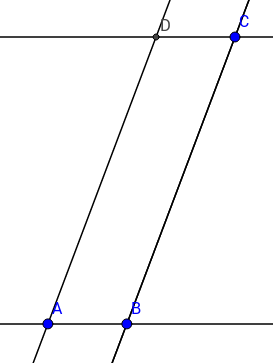
\includegraphics[width=1.56250in]{parallelogram.png}
Строим параллелограмм как на рисунке.
\(CD = AB\).

\begin{enumerate}
\def\labelenumi{\alph{enumi})}
\i
  Берём отрезок \(01\) и произвольную точку \(A\), не лежащую на нём. Проводим \(0A\). На луче \(0A\) начиная от точки \(0\) откладываем \(n\) равных отрезков произвольной длины. Пусть их концы, лежащие на \(0A\), есть \(A_1, \dots, A_n\) (считая от точки \(0\)). Проводим \(A_n1 =: A_n B_n\) и параллельно ей \(A_{n-1}B_{n-1}, \dots, A_1B_1\). По теореме Фалеса \(0B_1 = B_1B_2 = \dots = B_{n-1}1\). Сделав так для любого \(n\), получим все точки с рациональными координатами на \(01\), размножить на ось OX тривиально, получить так же поделенную ось OY тривиально, а т. к. любая точка однозначно задаётся проекциями и мы умеем строить перпендикуляры, можем строить любую точку с рациональными координатами.
\i
  Шестиугольник --- откладывая на окружности хорды длиной с радиус, треугольник --- по шестиугольнику, четырёхугольник --- строя перпендикуляр из центра окружности, в которую он вписан.
\i
  Отражение относительно осей.
\i
  Тривиально.
\i
  В экспоненциальной записи: \(z\omega = r_1e^{i\phi_1}r_2e^{i\phi_2}=(r_1r_2)e^{i(\phi_1 +\phi_2}\).
  Итого, надо научиться строить сумму углов и отрезок с длиной, равной произведению двух других. Сумма углов: тривиально.
  Произведение: пользуемся теоремой из геометрии о соотношении высоты прямоугольного треугольника со всякими другими отрезками (та, которая выводится из подобия).

  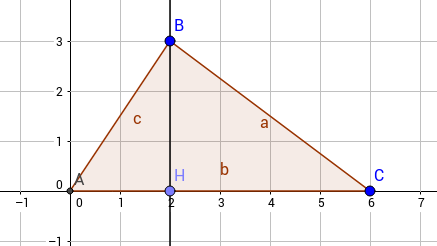
\includegraphics[width=2.08333in]{triangle.png}
  Взяв \(BH=h^2, AH=a^2, CH=b^2\), получим \(BH^2=AH\cdot CH \Then BH=ab\).
  Как строить \(a^2\) и \(b^2\)?
  Взяв \(BH=a^2, AH=1, CH=x\), получим \(a^2=1\cdot x \Then x=a^2\).
\end{enumerate}

\end{solution}

\begin{problem}[39 (9.12а)]
Докажите невозможность \bf{удвоения куба}, то есть построение куба объёма $2$, имея куб объёма $1$ с помощью циркуля и линейки.
\end{problem}

\begin{solution}
Задача сводится к построению циркулем и линейкой числа \(\sqrt[3]{2}\). Но \(\Q(\sqrt[3]{2})\) --- расширение степени 3 над \(\Q\), поэтому не существует башни промежуточных расширений размерности 2.

\bf{TODO: Больше объяснений!}
\end{solution}

\begin{problem}[40 (10.2)]
Пусть $\varphi: F \to F$ --- \it{автоморфизм поля} $F$ (изоморфизм поля на себя). 
a) Пусть $\mathrm{char} F =0$. Верно ли, что $\varphi$ сохраняет $\Q$? (то есть при $q\in\Q$ выполнено равенство $\varphi(q)=q$).
b) Пусть $\mathrm{char} F =p$. Верно ли, что $\varphi$ сохраняет $\Z_p$?
\end{problem}

\begin{solution}
\begin{enumerate}
\def\labelenumi{\alph{enumi})}
\i Автоморфизм переводит единицу в единицу: \(\phi(1) = 1\) по свойствам гомоморфизма.
Тогда \(\forall p \in \Z \Have \phi(p) = \phi(\ubrace{1+\dots+1}{p} = \ubrace{1+\dots+1}{p} = p\). Получили, что \(\Z\) сохраняется.

Тогда $\phi(2) = \phi(1+1) = \phi(1)+\phi(1)=1+1=2$.
И так далее. Получили, что $\Z$ сохраняется.

Если какой-нибудь элемент $\frac{a}{b} \in \Q$ перевёлся не в себя, то $\phi(\ubrace{\frac{a}{b}+\dots+\frac{a}{b}}{b}) = \ubrace{\phi(\frac{a}{b})+\dots+\phi(\frac{a}{b})}{b} \ne a$, т. е. в $\Z$ что-то перешло не в себя. Противоречие.
%Имеем: \(\frac{p}{q} \ubrace{\~}{\text{определение экв-ти}} \frac{pq^{-1}}{1} \ubrace{\~}{\text{изоморфизм}} pq^{-1}\)
%
%Тогда \(\phi(\frac{p}{a}) = \phi(pa^{-1}) = \phi(p)\ubrace{[\phi(a)]^{-1}}{\text{свойство гомоморфизма}} = pa^{-1} = \frac{p}{a}\)

\i Да, т. к. если \(m \in \Zp\), то \(\phi(m) = \ubrace{\phi(1)+\dots+\phi(1)}{m} = m\)
\end{enumerate}
\end{solution}

\begin{problem}[41 (10.4) (Lectures\_all.pdf задача 9.1, утв. 9.1)]
Пусть $F \subset K$ — расширение полей. Множество автоморфизмов $K$, оставляющих $F$ на месте, является группой и называется группой автоморфизмов и обозначается $\Aut_F(K) = \Aut([K : F])$.
a) $\Aut_F(K)$ — группа.
b) Пусть $H \subset \Aut_F(K)$ --- подгруппа. Тогда $K^H = \{x \in K \mid \forall h \in H \Have h(x) = x\}$ является полем, причём $K \supset K^H \supset F$.
\end{problem}

\begin{solution}
\begin{enumerate}
\def\labelenumi{\alph{enumi})}
\i Композиция автоморфизмов, сохраняющих \(F\), --- автоморфизм, сохраняющий \(F\) \(\Then\) замкнутость.

\(id\) --- нейтральный элемент.

Ассоциативность следует из свойств композиции.

Обратный существует, т. к. автоморфизм --- биекция. Обратный сохраняет \(F\).

\i Пусть \(a, b \in K^H, h \in H\). Тогда \(h(a + b) = h(a) + h(b) = a + b\), и поэтому \(a + b \in K^H\). Аналогично, \(ab \in K^H\). С другой стороны, \(h \in H \subset G\), и поэтому \(h\) сохраняет \(F\). Значит, \(F \subset K^H\).
\(K^H \subset K\) по определению.
\end{enumerate}
\end{solution}

\begin{problem}[42 (10.5)]
Опишите группы автоморфизмов $\Q(\sqrt[3]{2})$.
\end{problem}

\begin{solution}
\(\Q(\sqrt[3]{2}\) --- группа \(\{id\}\), т. к. все другие перестановки корней дают комплексные числа.

Знаем, что любой автоморфизм задаётся перестановкой корней минимального многочлена.

Пусть \(\phi\) --- авторморфизм. Тогда \(\phi(m_\gamma(\gamma)) = 0 \Then 0 = a_n \phi(\gamma)^m+\dots+a_0 \Then \phi(\gamma)\) --- корень \(m_\gamma\) \(\Then\) сопряжён с \(\gamma\).
\end{solution}

\begin{problem}[43 (11.1) (Lectures\_all.pdf теор. 11.1)]
a) Конечное поле характеристики $p$ состоит из $p^n$ элементов. 
b) Поле $F$ является полем разложения многочлена $x^{p^n}-x$. 
c) Cуществует единственное поле из $p^n$ элементов.
\end{problem}

\begin{solution}
\begin{enumerate}
\def\labelenumi{\alph{enumi})}
\i Так как \(K\) --- конечное расширение поля \(\Zp\), то \(K\) является n-мерным линейным пространством над \(\Zp\), и поэтому состоит из \(p^n\) элементов.
\i Пусть \(\alpha \in K, \alpha \ne 0\). Тогда \(\alpha^{p^n-1} = 1\). Следовательно, \(\alpha\) является корнем многочлена \(f\). Степень многочлена \(f\) равна \(p^n\), все элементы K являются его корнями. Ясно, что \(K\) --- минимальное поле, в котором \(f\) раскладывается на линейные множители. Следовательно, K --- его поле разложения.
\i Поле разложение многочлена \(f\) единственно с точностью до изоморфизма.
\end{enumerate}
\end{solution}

\begin{problem}[44 (11.2)]
Найдите все неприводимые многочлены (со стар. коэффициент $1$) степени $2$, $3$ над полем a) $\F_2$, b) $\F_3$.
\end{problem}

\begin{solution}
Выписываем все возможные многочлены и вычёркиваем те, которые разложимы.

\begin{enumerate}
\def\labelenumi{\alph{enumi})}
\i
  \(\F_2\):
  Неразложимые степени 1: x и x+1. Разложимые степени 2 --- какая-то комбинация многочленов степени 1. Оставшиеся --- неразложимы. Теперь смотрим всё возможные многочлены степени 3, которые можно получить, перемножая многочлены степени 1 и многочлены степени 2.

  \(\deg=2\): \(\s{x^2}, \ubrace{\s{x^2+1}}{(x+1)(x+1)}, \s{x^2+x}, x^2+x+1\)

  \(\deg=3\): \(\s{x^3}, \ubrace{\s{x^3+1}}{(x^2+1)(x^2+x+1)}, \s{x^3+x}, x^3+x+1, \s{x^3+x^2}, x^3+x^2+1, \s{x^3+x^2+x}, \ubrace{\s{x^3+x^2+x+1}}{(x^2+1)(x+1)}\)
\i
  \(\F_3\):
  Рассуждения аналогичны.

  \(\deg=2\): \(\s{x^2}, x^2+1, \ubrace{\s{x^2+2}}{(x+2)(x+1)}, \s{x^2+x}, x^2+x+1, \ubrace{\s{x^2+x+2}}{(x+1)(x+2)}, \s{x^2+2x}, x^2+2x+1, x^2+2x+2\)

  \(\deg=3\): \(\s{x^3}, \ubrace{\s{x^3+1}}{(x^2+1)(x^2+x+1)}, x^3+2, \s{x^3+x}, x^3+x+1, x^3+x+2, \s{x^3+2x}, x^3+2x+1, x^3+2x+2, \s{x^3+x^2}, x^3+x^2+1, x^3+x^2+2, \s{x^3+x^2+x}, \ubrace{\s{x^3+x^2+x+1}}{(x^2+1)(x+1)}, x^3+x^2+x+2, \s{x^3+x^2+2x}, x^3+x^2+2x+1, \ubrace{\s{x^3+x^2+2x+2}}{(x^2+2)(x+1)}, \s{x^3+2x^2}, x^3+2x^2+1, x^3+2x^2+2, \s{x^3+2x^2+x}, x^3+2x^2+x+1, \ubrace{\s{x^3+2x^2+x+2}}{(x^2+1)(x+2)}, \s{x^3+2x^2+2x}, \ubrace{\s{x^3+2x^2+2x+1}}{(x^2+2)(x+2)}, x^3+2x^2+2x+2\)
\end{enumerate}

\end{solution}

\begin{problem}[45 (11.3)]
Постройте поле из a) $4$; b) $8$; c) $9$ элементов.
\end{problem}

\begin{solution}

Для \(p^n\): \(F_{p^n} = \sfrac{F_p[x]}{(f(x))}\), где \(f(x)\) --- неприводимый многочлен степени n (пользуемся №33: $[\sfrac{F[x]}{(f(x))}:F] = n$). Итого, надо просто найти неприводимый многочлен над \(F_p\) степени \(n\). Как искать неприводимые многочлены рассказано в №44.

\begin{enumerate}
\def\labelenumi{\alph{enumi})}
\tightlist
\i
  \(4=2^2\)
  \(\F_4 = \sfrac{F_2[x]}{(x^2+x+1)} = \{0; 1;x;1+x\}\)
\i
  \(8=2^3\)
  \(\F_8 = \sfrac{F_2[x]}{(x^3+x^2+1)} = \{0; 1; x; x+1; x^2; x^2+1; x^2+x; x^2+x+1 \}\)
\i
  \(9=3^2\)
  \(\F_9 = \sfrac{F_3[x]}{(x^2+1)}\)
\end{enumerate}

Чтобы выписать элементы кольца явно, берём все возможные многочлены нужной степени над нужным полем и делим с остатком на многочлен, по которому факторизуем (факторизация в данном случае и есть деление с остатком).

\end{solution}

\end{document}
